\subsection{Kiểm thử các xử lý logic}

Để đảm bảo hệ thống hoạt động ổn định và chính xác, các xử lý logic của hệ thống cần được kiểm thử kỹ lưỡng. Các kiểm thử này sẽ giúp phát hiện và sửa chữa các lỗi trong mã nguồn, đảm bảo rằng các chức năng của hệ thống hoạt động như mong đợi. Các kiểm thử này bao gồm kiểm thử đơn vị (Unit Testing) và kiểm thử API (API Testing).
\subsubsection{Kiểm thử đơn vị}


\textbf{Phạm vi kiểm thử}

Phạm vi kiểm thử đơn vị cho ứng dụng Smart Gallery bao gồm kiểm thử các hàm xử lý và các lớp xử lý logic của 2 server labeling ảnh và server tạo video. 

\textbf{Môi trường kiểm thử}

Môi trường kiểm thử cho các xử lý logic gồm có: 
\begin{itemize}
    \item JestJS\cite{jestJS}: là một công cụ được sử
    dụng để kiểm thử đơn vị được tích hợp sẵn trong NodeJs.
    \item pytest\cite{pytest}: là một thư viện kiểm thử đơn vị mạnh mẽ và linh hoạt cho Python. Kết hợp song song với unittest\cite{unittest}, pytest giúp kiểm thử các hàm xử lý logic của server labeling ảnh.
\end{itemize}

\textbf{Kết quả kiểm thử}

Độ phủ và kết quả kiểm thử xử lý logic như Hình \ref{fig:jest-testing} và Hình \ref{fig:pytest-testing}.

\begin{figure}[H]
    \centering  
    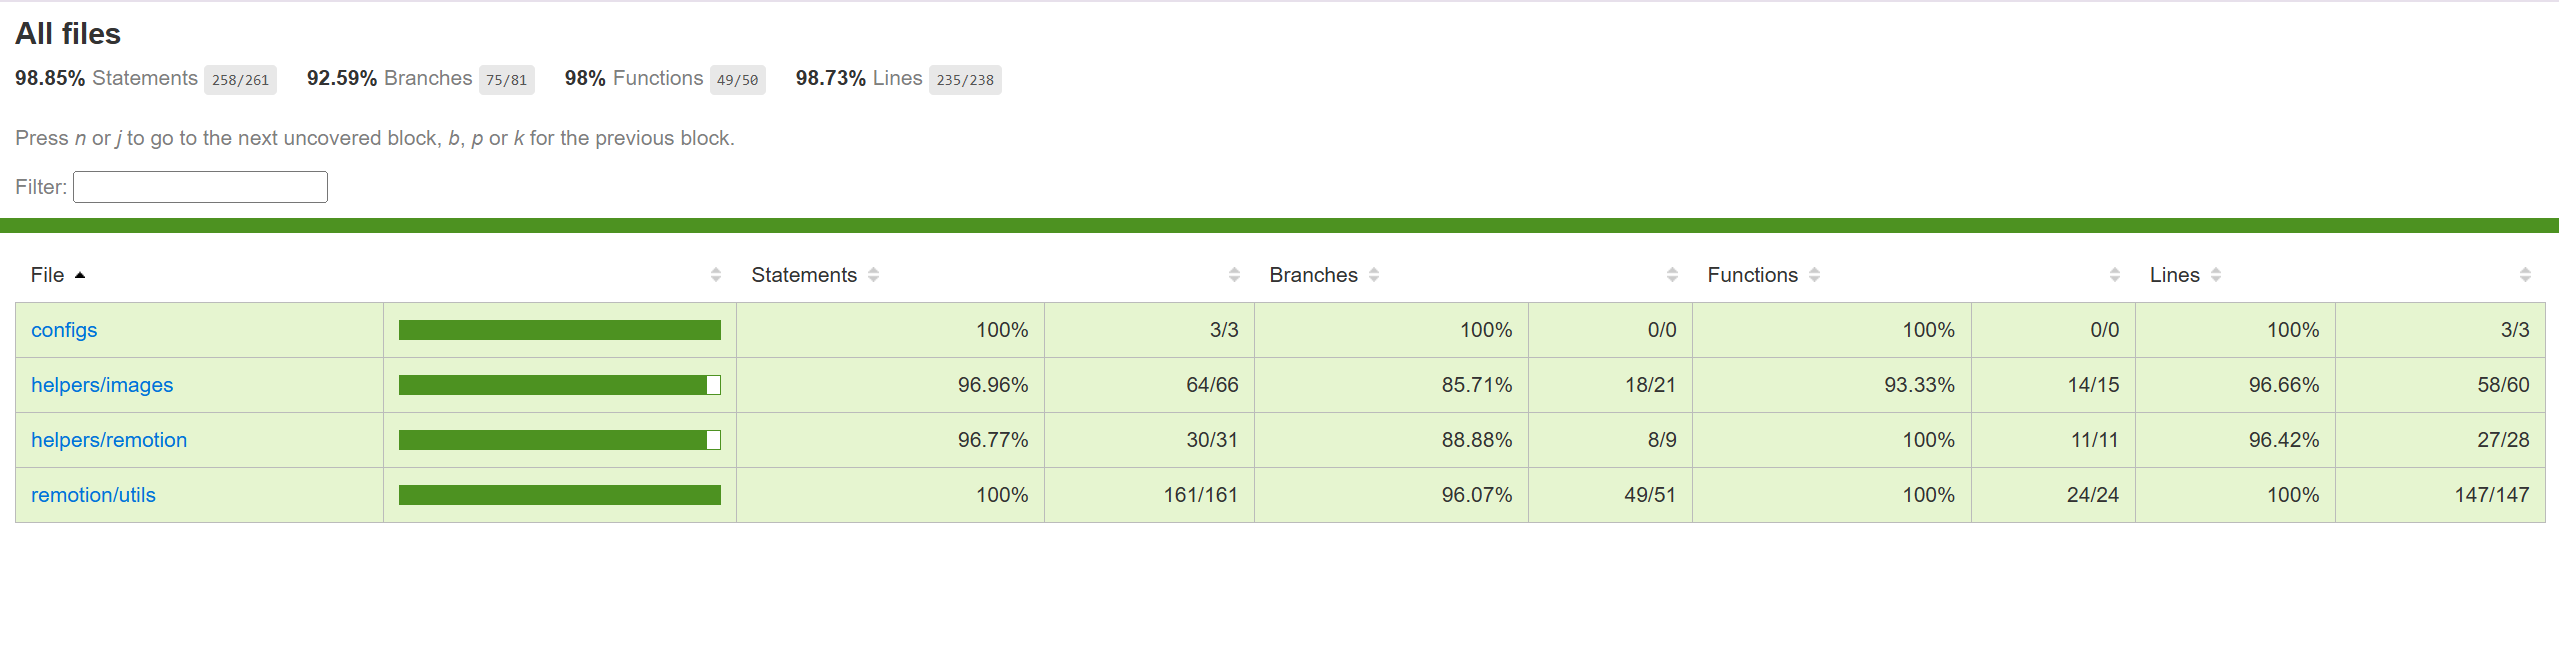
\includegraphics[width=1\textwidth]{figures/c4/4-3/jest.png}
    \caption{Độ phủ kiểm thử xử lý logic với JestJS.}
    \label{fig:jest-testing}
\end{figure}

% \begin{figure}[H]
%     \centering  
%     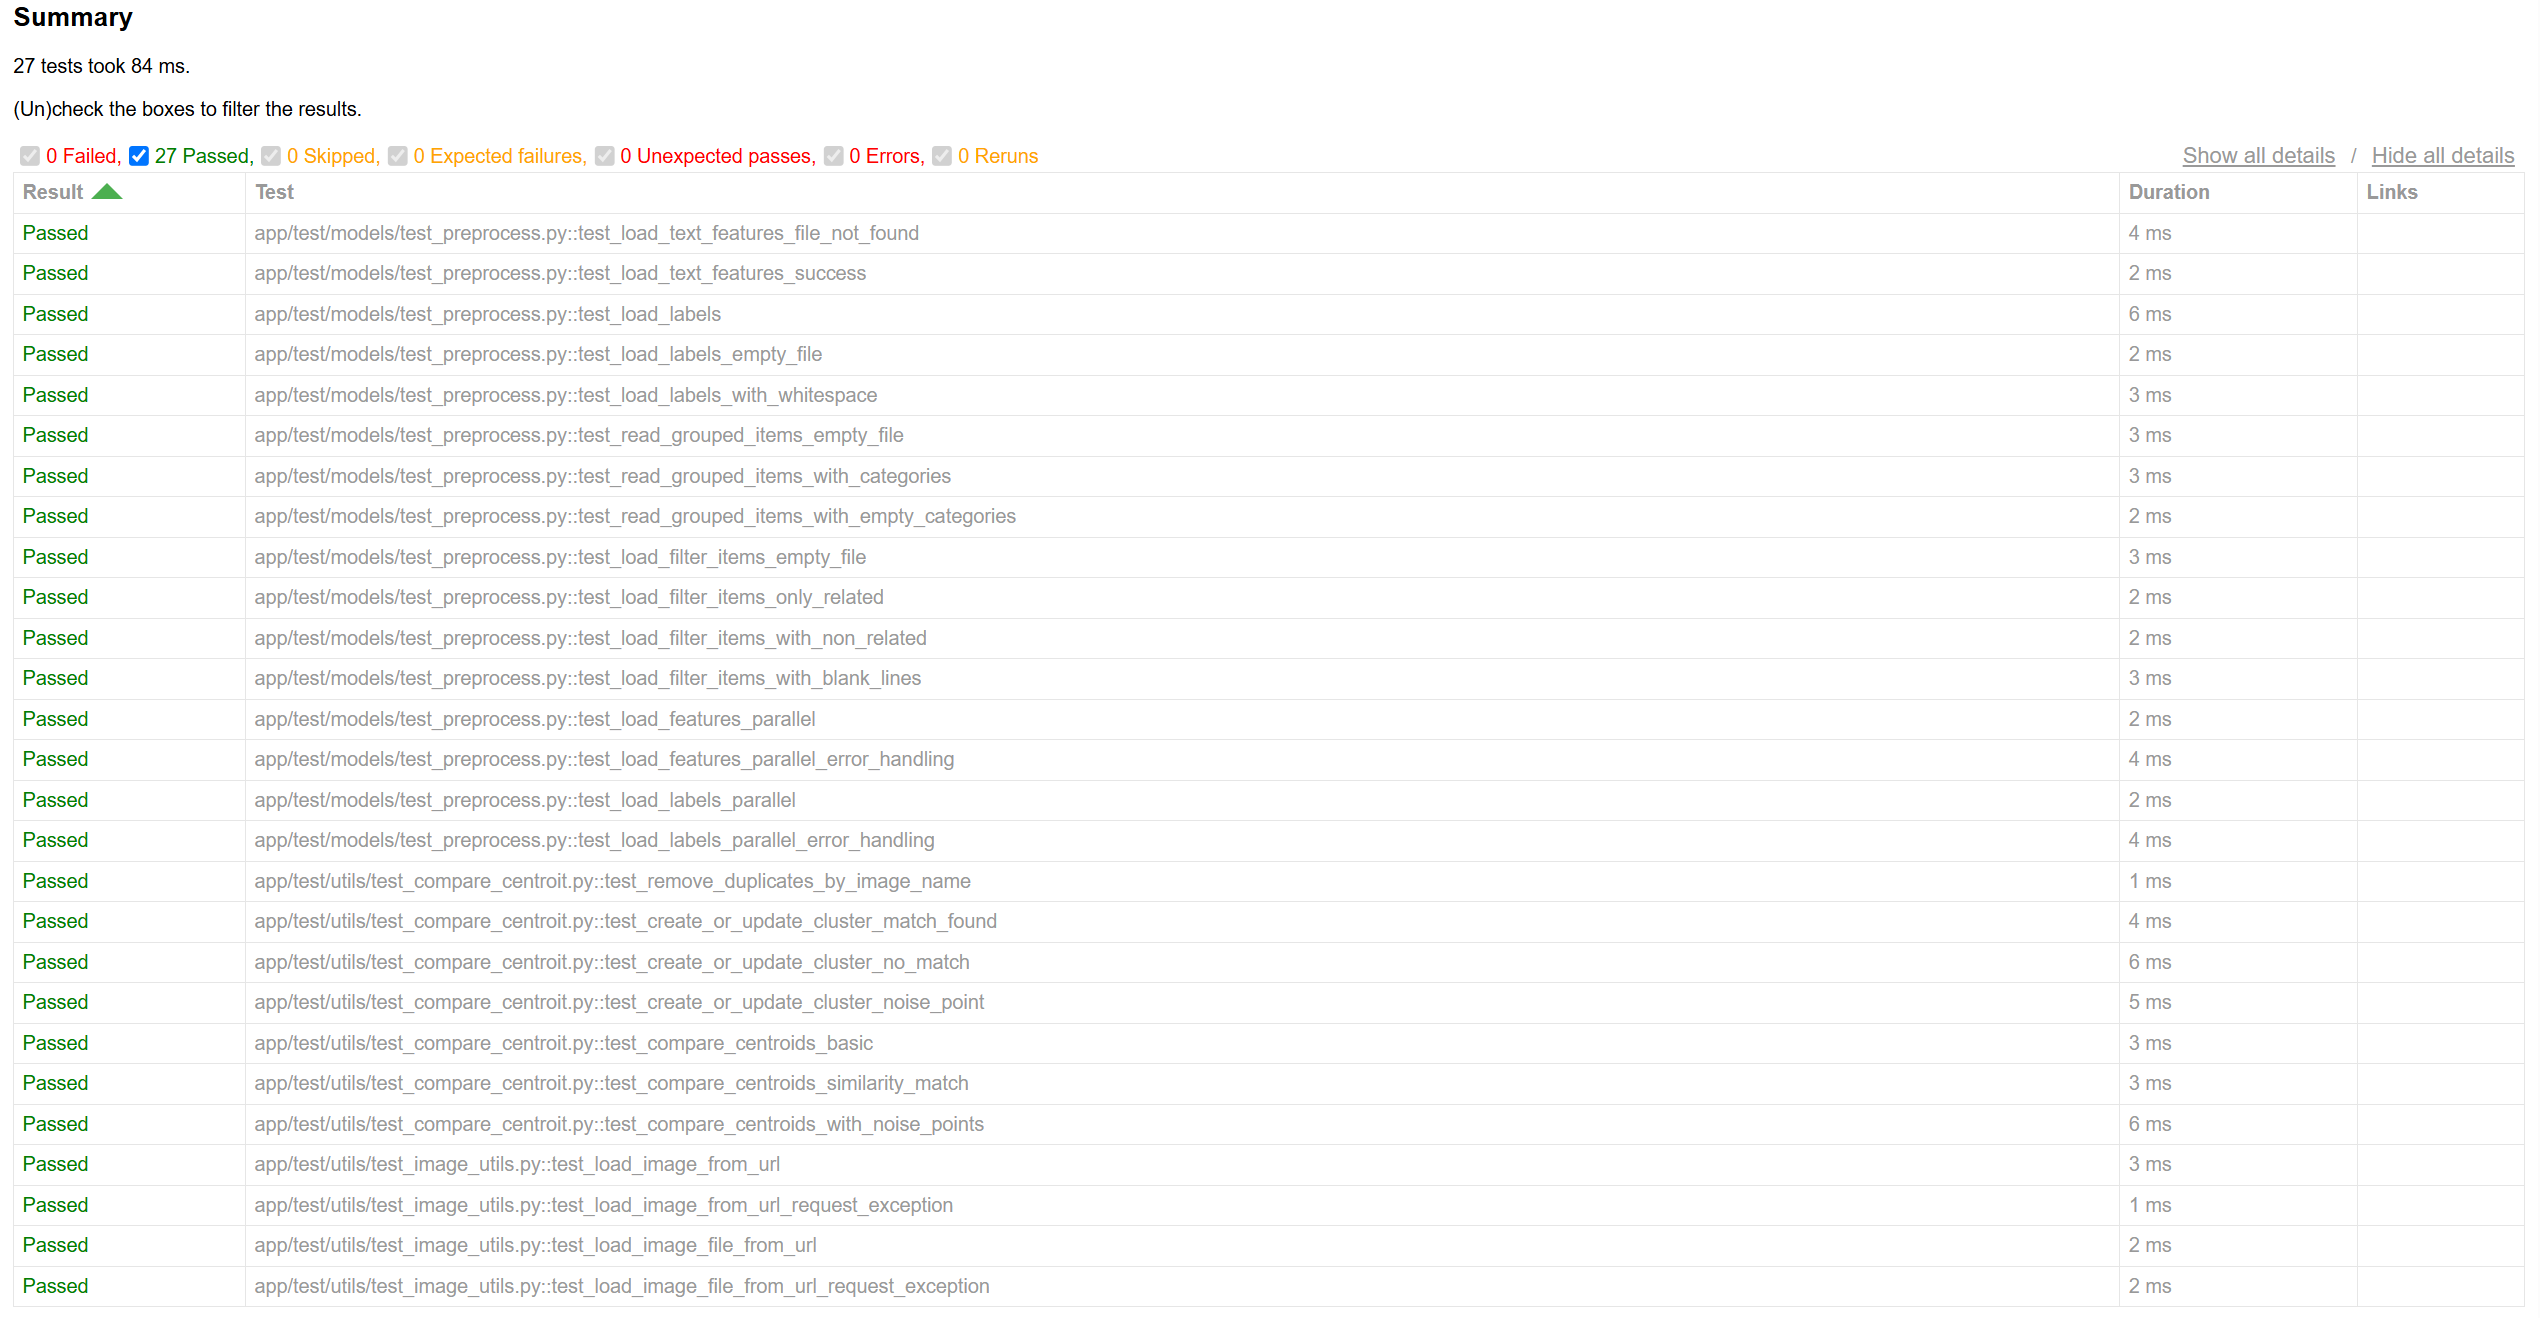
\includegraphics[width=1\textwidth]{figures/c4/4-3/pytest.png}
%     \caption{Kết quả các ca kiểm thử đơn vị với Pytest.}
%     \label{fig:pytest-coverage}
% \end{figure}

\begin{figure}[H]
    \centering  
    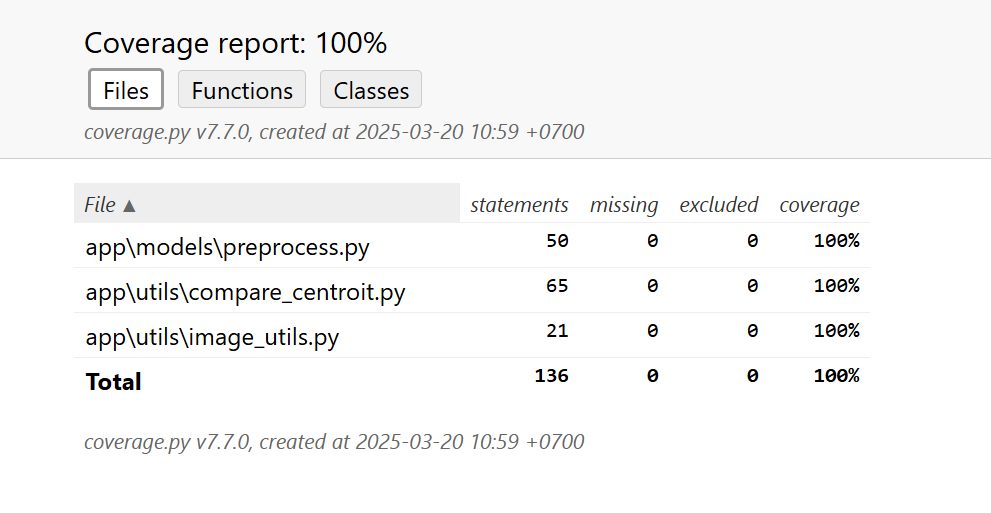
\includegraphics[width=1\textwidth]{figures/c4/4-3/pytest_2.png}
    \caption{Độ phủ kiểm thử xử lý logic với pytest.}
    \label{fig:pytest-testing}
\end{figure}


\subsubsection{Kiểm thử API}

Chi tiết các ca kiểm thử (miêu tả, input và output) được mô tả tại folder "[test]" tại đây\footnote{\url{http://bit.ly/42y7KyF}}. 
Và Hình \ref{fig:postman} dưới đây mô tả các API endpoint được kiểm thử với Postman\cite{postman}.  

\begin{figure}[H]
    \centering  
    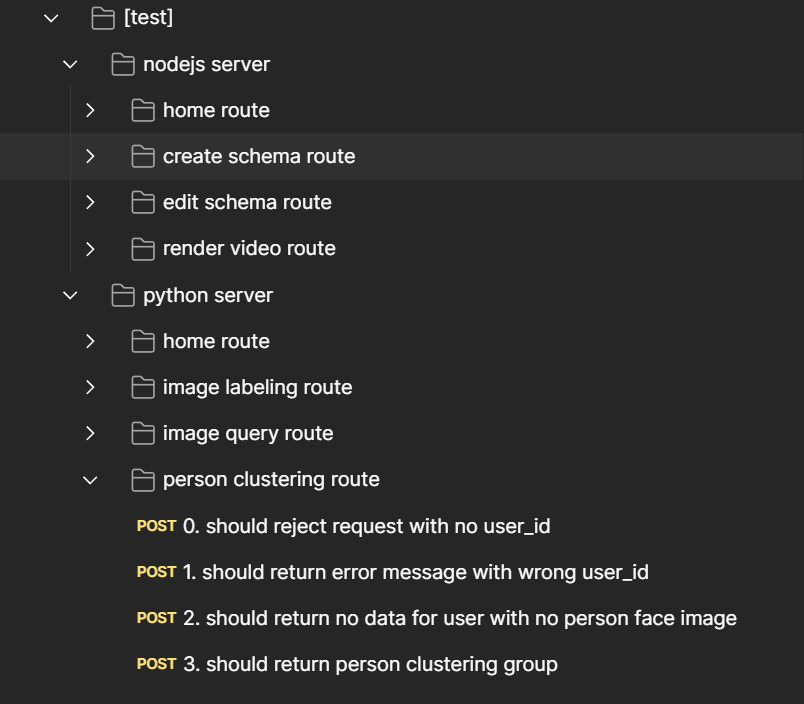
\includegraphics[width=0.7\textwidth]{figures/c4/4-3/api.png}
    \caption{Các API endpoint được kiểm thử với Postman.}
    \label{fig:postman}
\end{figure}


Bảng 4.1 dưới đây mô tả một số kịch bảng kiểm thử API chính cho ứng dụng. 

\small
\begin{xltabular}{\textwidth}{|c|p{2cm}|X|X|c|}
    \caption{Các kịch bản kiểm thử API chính} \label{tab:api-test-cases} \\
    \hline
    \textbf{STT} & \textbf{API} & \textbf{Ca kiểm thử} & \textbf{Kết quả kỳ vọng} & \textbf{Tình trạng} \\
    \hline
    \endfirsthead
    
    \multicolumn{5}{c}{\tablename\ \thetable{} (tiếp theo)} \\
    \hline
    \textbf{STT} & \textbf{API} & \textbf{Ca kiểm thử} & \textbf{Kết quả kỳ vọng} & \textbf{Tình trạng} \\
    \hline
    \endhead
    
    \hline \multicolumn{5}{r}{\textit{Tiếp trang sau}} \\
    \endfoot
    
    \hline
    \endlastfoot
    
    \multirow{3}{*}{1} & \multirow{3}{=}{\centering API tạo kịch bản video} & Tạo kịch bản video từ 5 hình ảnh hợp lệ & Hệ thống tạo được kịch bản, trả về mã 201 và thông tin kịch bản vừa tạo & Đạt \\
    \cline{3-5}
     & & Tạo kịch bản video không kèm theo ảnh & Hệ thống trả về mã lỗi 400 và thông báo cần gửi kèm danh sách ảnh & Đạt \\
    \cline{3-5}
    & & Người dùng chưa xác thực tạo kịch bản video & Hệ thống trả về mã lỗi 400 và thông báo cần xác thực & Đạt \\
    \hline
    \multirow{2}{*}{2} & \multirow{2}{=}{\centering API sửa kịch bản video} & Thay đổi tiêu đề video & Hệ thống thay đổi kịch bản, trả về mã 201 và thông tin kịch bản vừa được cập nhật & Đạt \\
    \cline{3-5}
     & & Thay đổi kịch bản video với params sai định dạng & Hệ thống trả về mã lỗi 400 và thông báo cần gửi yêu cầu đúng định dạng & Đạt \\
    \hline
    \multirow{3}{*}{3} & \multirow{3}{=}{\centering API tạo video} & Tạo video với kịch bản có sẵn & Hệ thống trả về ID của video cùng mã 201 & Đạt \\
    \cline{3-5}
     & & Tạo video không kèm theo token người dùng & Hệ thống trả về mã lỗi 400 và thông báo cần xác thực & Đạt \\
    \cline{3-5}
     & & Yêu cầu tạo cùng 1 video 2 lần & Hệ thống trả về mã lỗi 400 và thông báo lỗi video đang được tạo & Đạt \\
    \hline
    \multirow{2}{*}{4} & \multirow{2}{=}{\centering API tìm kiếm hình ảnh} & Tìm kiếm với từ khóa & Hệ thống trả về danh sách hình ảnh phù hợp và mã 200 & Đạt \\
    \cline{3-5}
     & & Người dùng chưa xác thực yêu cầu tìm kiếm với từ khóa & Hệ thống trả về mã lỗi 400 và thông báo cần xác thực & Đạt \\
    \hline
    \multirow{2}{*}{5} & \multirow{2}{=}{\centering API phân nhóm khuôn mặt} & Phân nhóm khuôn mặt với danh sách ảnh không có khuôn mặt & Hệ thống trả về danh sách rỗng và mã 200 & Đạt \\
    \cline{3-5}
     & & Phân nhóm khuôn mặt với danh sách 20 ảnh chứa 40 khuôn mặt & Hệ thống trả về danh sách nhóm khuôn mặt tương tự và mã 200 & Đạt \\
    \hline
    \multirow{3}{*}{6} & \multirow{3}{=}{\centering API gán nhãn ảnh} & Phân nhóm khuôn mặt với danh sách ảnh không có khuôn mặt & Hệ thống trả về danh sách rỗng và mã 200 & Đạt \\
    \cline{3-5}
     & & Gán nhãn 1 ảnh & Hệ thống trả nhãn của ảnh và mã 200 & Đạt \\
    \cline{3-5}
     & & Gán nhãn nhiều ảnh & Hệ thống trả về mảng nhãn ảnh và mã 200 & Đạt \\
    \hline
\end{xltabular}

